\section{Mise en place de l'infrastructure}
\subsection{Accès ssh à la raspberry pi}
La raspberry pi a été configurée avec l'adresse IP 192.168.1.2. Il faut configurer l'ordinateur avec une adresse IP 192.168.1.x et le masque réseau 255.255.255.0, cela permet aux deux appareils de communiquer.
\subsubsection{Configuration pour VirtualBox}
Pour partager la connexion dans une machine virtuelle, il faut régler le réseau en \textit{Accès par pont} comme le montre l'image ci-dessous.
\begin{figure}[H]
	\begin{center}
		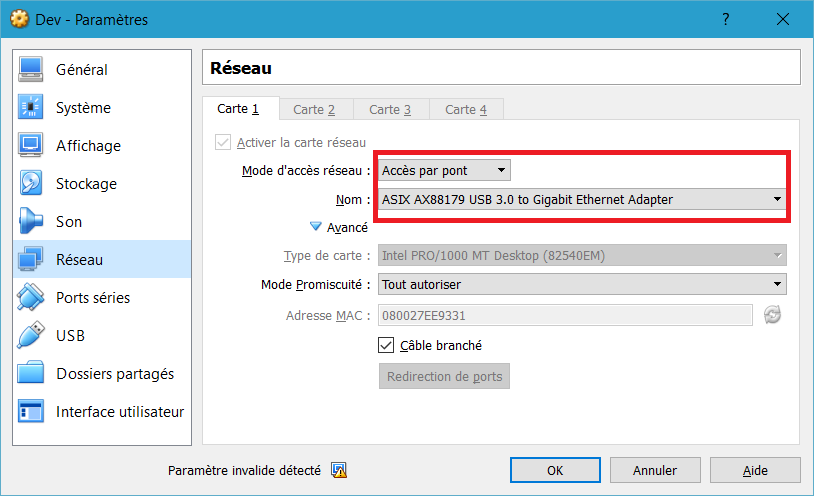
\includegraphics[width=14cm]{img/vmConfig1.png}
		\caption{Configuration de la carte réseau}
		\label{evLinuxConfig1}
	\end{center}
\end{figure}
Il faut également couper la connexion wifi de l'ordinateur, cela lui permettra de se brancher sur la connexion Ethernet.\\
La dernière étape consiste à aller modifier l'adresse IP de la machine virtuelle en changeant les paramètres IPv4. Nous lui avons attribué l'adresse 192.168.1.100.
\begin{figure}[H]
	\begin{center}
		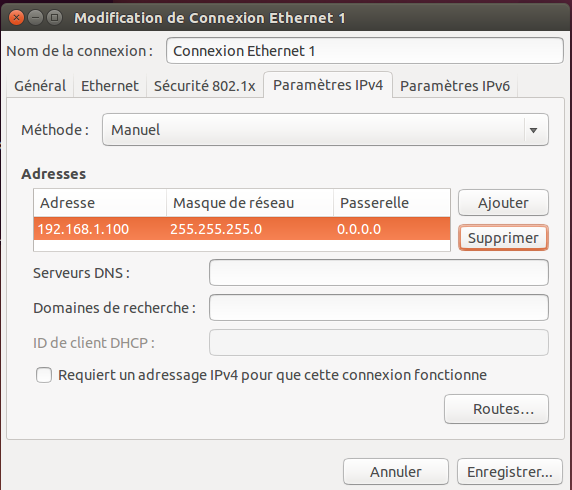
\includegraphics[width=14cm]{img/vmConfig2.png}
		\caption{Changement de l'adresse IP}
		\label{evLinuxConfig2}
	\end{center}
\end{figure}
Il est maitenant possible d'accéder à la raspberry pi par ssh:
\begin{lstlisting}
	$ ssh pi@192.168.1.2
	The authenticity of host '192.168.1.2 (192.168.1.2)' can't be established.
	ECDSA key fingerprint is 80:b2:dc:9d:a5:4e:e7:1a:32:60:11:1c:8b:44:39:0e.
	Are you sure you want to continue connecting (yes/no)? yes
	Warning: Permanently added '192.168.1.2' (ECDSA) to the list of known hosts.
	pi@192.168.1.2's password: 
	...
	pi@raspberrypi:~ $ 
\end{lstlisting}

